\section*{Dynamische Terminbuchung}
Das Frontend wurde als Single Page Anwendung (SPA) geschrieben. Eine SPA ermöglicht es, 
Inhalte dynamisch nachzuladen, ohne dass die gesamte Seite neu geladen werden muss. Dies 
sorgt für eine schnelle und unterbrechungsfreie Benutzererfahrung, da die Anwendung stets 
direkt auf Nutzerinteraktionen reagieren kann.
Ein zentraler Bestandteil des Frontends ist die dynamische Verwaltung von Impfterminen. 
Nutzer können über die Anwendung verfügbare Termine einsehen, Buchungen vornehmen und 
bestehende Reservierungen verwalten. Diese Funktionen werden über verschiedene 
JavaScript-Dateien gesteuert.
Beim Aufruf der Terminbuchungsseite wird automatisch eine asynchrone Anfrage mittels AJAX
an das Backend gestellt, um die aktuell verfügbaren Termine in einem Kalender abzurufen. 
Dadurch werden dem Nutzer nur tatsächlich buchbare Slots angezeigt. Zusätzlich wird 
sichergestellt, dass bereits gebuchte oder abgelaufene Termine nicht mehr auswählbar sind.
%\begin{center}
%  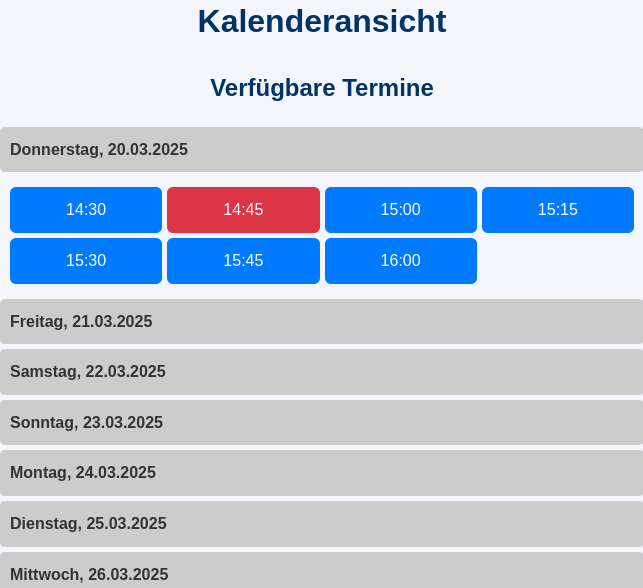
\includegraphics[width=0.95\linewidth, height=0.45\textheight, keepaspectratio]{src/abbildungen/kalenderansicht.png}
%  \captionof{figure}{Kalenderansicht}
%\end{center}
Ein wesentlicher Vorteil dieses Konzepts ist die verbesserte Performance der Anwendung. 
Statt bei jeder Benutzeraktion eine komplette neue Seite zu laden, werden nur die 
tatsächlich benötigten Daten nachgefordert. Dies reduziert nicht nur die Ladezeiten, 
sondern verringert auch die Serverlast, da weniger Daten übertragen werden müssen. 
